\documentclass[11pt]{article}
\usepackage[letterpaper,top=4cm,bottom=4cm,left=3cm,right=3cm,marginparwidth=1.75cm]{geometry}

\usepackage{authblk}
\usepackage{color, colortbl}
\usepackage[dvipsnames]{xcolor}
\usepackage[backend=biber,style=numeric,sorting=none]{biblatex} % bibliography
\usepackage[toc,page]{appendix} % Appendixes
\addbibresource{bibliography.bib} % bibliography

\usepackage{fancyhdr} % Add headers
\usepackage{lastpage} % Get total pages in document

\usepackage{setspace}


\usepackage{algorithm}
\usepackage{algpseudocode}

% begin header configuration
\pagestyle{fancy}

% Start fancyhdr settings
\fancyhf{}
\fancyhead[L]{\leftmark}  % section
%\fancyhead[R]{\rightmark}  % subsection
\fancyfoot[C]{\thepage} 
\cfoot{\thepage\ of \pageref{LastPage}}
% End fancyhdr settings
% End header configuration

\usepackage{amsmath} % Extra math functions
\usepackage{lipsum}  

\definecolor{RowHeader}{rgb}{0.827,0.827,0.827}
\definecolor{high}{rgb}{0.7,0.5,0.5}
\definecolor{severe}{rgb}{1,0.2,0.2}
\definecolor{dkgreen}{rgb}{0,0.6,0}
\definecolor{string}{rgb}{0.3,0.6,0.3}
\definecolor{gray}{rgb}{0.5,0.5,0.5}
\definecolor{mauve}{rgb}{0.58,0,0.82}
\definecolor{lightgray}{rgb}{0.95,0.95,0.95}

\usepackage{tabularx} % Better tables
\newenvironment{ctabularx}[1]{% or whatever name you like
   \rowcolors{1}{}{lightgray}%
   \tabularx{#1}%
  }{%
   \endtabularx
}


% Center captions
\usepackage{caption}
\captionsetup{font=footnotesize}
\captionsetup{justification=centering, margin=1cm}

\usepackage{graphicx} % Required for inserting images
\usepackage{float} % Required for inserting images

\usepackage[hidelinks]{hyperref} % Generate clickable links in PDF (cites, references etc)
%\usepackage{hyperref} % Generate clickable links in PDF (cites, references etc)
\usepackage{booktabs} % To thicken table lines



\usepackage{listings}

\lstdefinestyle{base} {
  aboveskip=3mm,
  belowskip=3mm,
  showstringspaces=false,
  columns=flexible,
  basicstyle={\small\ttfamily},
  numbers=none,
  numberstyle=\tiny\color{gray},
  keywordstyle=\color{blue},
  commentstyle=\color{dkgreen},
  stringstyle=\color{string},
  breaklines=true,
  breakatwhitespace=true,
  tabsize=3,
  numbers=left,
  stepnumber=1,
}

% CSharp
\lstdefinestyle{base_csharp} {%
  language=[Sharp]C, 
  morekeywords={nint, unit, nuint, var, await},
  style=base
}
\lstnewenvironment{csharp}{%
    \lstset{%
        style=base_csharp,
    }
}{}


% Java
\lstdefinestyle{base_java} {%
  language=Java, 
  style=base
}

\lstnewenvironment{java}{%
    \lstset{%
        style=base_java,
    }
}{}

% Typescript
\lstdefinestyle{base_typescript} {
  style=base,
  keywords={abstract, any, as, boolean, break, case, catch, class, console, 
    const, continue, debugger, declare, default, delete, do, else, enum, export, 
    extends, false, finally, for, from, function, get, if, implements, import, in, 
    infer, instanceof, interface, keyof, let, module, namespace, never, new, null, 
    number, object, package, private, protected, public, readonly, require, return, 
    set, static, string, super, switch, symbol, this, throw, true, try, type, typeof, await,
    undefined, unique, unknown, var, void, while, with, yield},
  morecomment=[s]{/*}{*/},
  morestring=[b]',
  morestring=[b]",
  morestring=[b]`,
  sensitive=true
}

\lstnewenvironment{typescript}{%
    \lstset{%
        style=base_typescript,
    }
}{}

\lstdefinestyle{yaml} {
  style=base,
  keywords={true,false,null,y,n},
  comment=[l]{\#},
  morestring=[b]',
  morestring=[b]",
  sensitive=true
}

\newcommand{\lb}[0]{\\ \\}

\title{Semantic Versioned SDK Generation: Streamlining Cross-Language Development}

\onehalfspace
\begin{document}

\author{Kristian, Jørgensen}

\begin{titlepage}
    \centering

    \vspace*{1cm}
    {
    \Huge
    Master Thesis
    
    \vspace*{0.2cm}
    \Large
    Master of Science in Engineering
    }
    
    \vspace*{2cm}

    \linespread{2.0}
    \huge\textbf{
        Semantic Versioned SDK Generation:
        Streamlining Cross-Language Development
    }
    \normalsize
    \linespread{1.0}

    \vspace{2,5cm}

    \linespread{1.2}
    \Large
    Kristian Jørgensen \\
    \large
    The Faculty of Engineering \\ 
    The Maersk Mc-Kinney Moller Institute \\ 
    University of Southern Denmark \\
    \normalsize
    \linespread{1.0}

    \vspace{1,5cm}

    \textbf{Supervisor:} Torben Worm - \texttt{tow@mmmi.sdu.dk} \\
    \textbf{Co-supervisor:} Aslak Johansen - \texttt{asjo@mmmi.sdu.dk}

    \vspace{1cm}
    
\includegraphics[width=0.3\textwidth]{figures/assets/sdu.png}

    \vspace{1cm}
    %\today
    June, 2024
\end{titlepage}

% \section*{Problemformulering}

\textbf{Hypetese} \\
By automating the conversion of data objects between languages, developers can both save time and reduce bugs, when developing an SDK.
\\ \\ 
\textbf{Problemformulering} \\
How can data transfer in a cross-language project be automated?

\begin{itemize}
    \item What is the need for this automation?
    \item What procedures are there currently?
    \item How can type definitions be ensured?
\end{itemize}

\subsection*{Notes}
\begin{itemize}
    \item Hvordan kan man lave cross-language software development?
    \item Hvordan kan man reducer tiden?
    \item Hvad får man ud af at gøre det?
    \item Hvad findes der i forvejen?
    \item Hvordan kan man gøre det tilgængeligt for alle
    \item 
\end{itemize}
% \section*{Notes}

\subsection*{Articles}
\begin{itemize}
    \item From Rasmus: \href{https://github.blog/2024-01-03-our-move-to-generated-sdks/}{Our move to generated SDKs}
\end{itemize}

\subsection*{Thoughts}
\begin{itemize}
    \item \textbf{Default project}: The SDK should be generated on top of a default project, where all the required files are.
    For Java, this could be a Java 8 maven project, with e.g. JetBrains nullable annotations
    For Typescript, this could be an NPM module, with some basic things installed.
    Access Modifier, Type, Name, Value 

    \item \textbf{Variable declarations patterns} Different languages declare variables differently.
    Java, C\#, Python, TypeScript, Go, Rust
    \hyperlink{https://blogger.googleusercontent.com/img/b/R29vZ2xl/AVvXsEjuc3AMG0GuHzqNIR1eLR4h5hTY-DJBgT9LCXziFdJMHiQzRC8L5_5zBrTUuujObkfBtcfyA8XmqK7JbY-vGf-i2M4Fx2Nn8nT6I_9rw0Qg-hw3T40Ha40qjA82Aqs8TLLz1Z5XEJdXE6rpWLQnMc3agYGDKRKda4C5yQnVUQKTWIlyz76rizvgJXNH/s608/2022-12-04_110650.png}{Definations}
    
    \item \textbf{Naming conventions} camelCase, PascalCase, snake\_case, kebab-case \\

    \[Name(carnonical: "IoStream")\]

    \item \textbf{Variable declerations}
    
    \item \textbf{Version Control} An option to export the SDK and give it an id. When a new change is published, it will check if there is any changes from the current SDK.
    Furthermore, an option to detect if the change was a breaking change, e.g. changing a route, removing an element from the body, changing a route signature
    
    \item \textbf{OpenApi} Check if the code should look thru the code, or take input from OpenAPI (or similar) and generate from that.
    Note. Does not support generics, inheritence or polymopishm. \href{https://document360.com/blog/open-api/}{Source}
    
    \item \textbf{Type Serilizer} It should be possible to create a custom sterilizer for each type.
    The sterilizer should have different options, such as required imports (which are different for each language.
    An option could be having it extend the different languages, e.g. "MySerlizier : JavaSerlizier, TypeScriptSerlizier"

    \item \textbf{Template engine} Scriban, Cottle, Fluid \hyperlink{https://r3c.github.io/cottle/benchmark.html}{Cottle benchmark}
    
    \item \textbf{Keep it simple} Pas på med ekstra features. F.eks. property type. Det er fint til produktet, men giver intent akademisk

    \item \textbf{Roslyn} Compile time code anylse ting ting.
https://github.com/Digizuite/digizuite.core/tree/feature/sdk-generation/SourceGenerators/SdkLowLevelGenerator

    \item \textbf{Java implementation} Compile time code anylse ting ting.
        \begin{itemize}
            \item \textbf{Maven} - Automatic getter / setter / constructor
            \item \textbf{Lombok} - Automatic getter / setter / constructor
            \item \textbf{Retrofit} - Automatic HTTP client
        \end{itemize}

   \item \textbf{Standard}
\begin{verbatim}
    endpoints [{
        url: "localhost:/api/users/{userId}",
        placeholders [{
            name: "userId",
            type: "number"
        }],
        parameters: [{
            name: "deprecated",
            type: "boolean"
        }],
        body: {
        
        }
    }]
\end{verbatim}

    \item \textbf{Planning} \hyperlink{https://tree.nathanfriend.io/}{Website}
    \begin{verbatim}
Master Theisis (code part) [27.5 days]
  Generate DTOs [21]
    Default projects [1.5 day]
      Versioning - 0.5 days]
      Package Manager - 0.5 days
      Packages - 0.5 days
    Runtime vs compile time [6.5 days]
      Reflection [1.5 days]
        Understanding - 0.5 days
        Testing - 1 day
      Ryslin [5 days]
        Understanding - 2 days
        Testing - 2 days
        AST - 1 day
    Template Engine [3 days]
      - Research [2 days]
      - Testing [1 day]
    Creating the converter [8 days] [Blockeb by: Template Engine, Runtime vs compile time, default projects]
      Basic model [4 days]
        Mapping: 2 days
        Convert to Java: 1 day
        Convert to TS: 1 day
      Inheritance - [2 days]
        Mapping: 1 day
        Java: 0.5. days
        TS: 0.5 day
      Generics - [2 days]
        Mapping: 1 day
        Java: 0.5 days
        TS: 0.5 day
    Configuration [2 days]
      JSON parsers [0.5 days]
      Versions [0.5 days]
      Property names [1 day]
        Default [0.5 days]
        Custom [0.5 days]
          System.Text.Json
          Newtonsoft
      Custom serilizer [1 day]
      
  Version Validation [2.5 days]  [Blockeb by: Creating the converter]
    Defining rules [0.5 day]
    Implementing rules [2 days]
  Generate interfaces [4 days] [Blockeb by: Creating converter]
    Creating template [1 day]
      Java [0.5 days]
      TS [0.5 days]
    Creating model [2 days]
    Testing [1 day]
  Implementing interfaces [Wont do]
    Authentication
    Rate limit
    Errors
    \end{verbatim}
    

\begin{csharp}
// Variable
public string MyVariable = "Hello World!";

// Fuction
public string MyMethod(sting arg)
{
  // body
}
\end{csharp}

\begin{java}
// Variable
public String myVariable = "Hello World!";

// Fuction
public String myMethod(sting arg)
{
  // body
}
\end{java}

\begin{typescript}
// Variable
myVariable: string = "Hello World!";

// Fuction
function myMethod(arg: string): string
{
  // body
}
\end{typescript}


\end{itemize}



\section*{Abstract}
This project aims to automate the conversion of Data Transferable Objects (DTOs) between different programming languages, eliminating a time-consuming task for developers and reducing errors that may occur in manual conversion. 
The approach involves creating a schema that details the structure of all DTOs, which can be converted into Software Development Kits (SDKs). This schema can be auto-generated by a Schema Provider, compared to previous versions by a Diff Checker, and converted into an SDK by a Schema Consumer.
\newline\newline
The report presents a prototype demonstrating this approach's feasibility. While the prototype shows promising results, further work is required to adapt this solution to real-world scenarios. Overall, this project has the potential to significantly reduce development time and effort, and minimize bugs associated with manual DTO conversion.
\tableofcontents
\section*{Vocabulary}
\begin{itemize}
  \item \textbf{DTO}: Data Transferable Object \\
  The definition for a strongly typed object. Often referred to as a \textit{Plain Old (Java / C\#) Object} in each retrospective language. \\
  \textit{Synonyms: Data Structure, Model}
  
  \item \textbf{SDK}: Software Development Kit \\
  A dependency other developers can include in their project, to gain access to code created by others. This could include DTOs and services to communicate with their API.
  
  \item \textbf{API}: Application Programming Interface  \\
  A standardized way to communicate with an application.
  
  \item \textbf{Project}: A code repository, containing a single namespace.
  
  \item \textbf{Solution}: Like a \textit{Project}, a solution is a code repository but contains multiple projects instead of just a single one.

\end{itemize}
\section{Introduction \label{sec:introduction}}
Modern software systems are often composed of different languages. This is especially true for a microservice architecture. To effectively communicate between these services, developers often use Data Transferable Objects (DTO), which describe exactly how the data structure looks. These DTOs can be used in a RESTful API, in a message bus, in socket communication or much more. This means they are widely used, and lay the standard for the data.
When developing within the same language, a Software Development KIT (SDK) can be created and published, allowing other team members to have access to the same DTO, ensuring they have all properties defined in their code base, and can access it all.
However, when switching between languages, this is no longer possible, as they cannot use an SDK for another language. To solve this, developers often undertake the task of duplicating the classes in multiple languages, having a strictly typed SDK for each language they use in development. 
This project aims to eliminate this manual conversion task.

\subsection{How the DTOs are used in code spaces}
A DTO is essentially a class structure, where properties are defined.
They do not include any business logic, which is commonly associated with classes in Object-Oriented Programming (OOP). Instead, they focus solely on encapsulating data.
Listing \ref{code:exmaple_dto} shows an example of two DTOs, defined in C\#
\begin{lstlisting}[caption={Example of a C\# DTO}, label={code:exmaple_dto}, style=base_csharp]
public class PersonDto
{
    public string FirstName { get; set; } 
    public string LastName { get; set; } 
    public DateOnly Birthday { get; set; } 
    public string AddressDto { get; set; } 
}

public class AddressDto
{
    public string Road { get; set; } 
    public int Number { get; set; } 
    public int ZipCode { get; set; } 
}
\end{lstlisting}
\noindent
When a DTO has been defined, it can then be used in a project.
Listings \ref{code:http_example_csahrp} and \ref{code:http_example_typescipt} show respectively how DTOs can be used in C\# or TypeScript when calling a RESTful API.
This is only one of the uses for these DTOs. 
In practice, they can be used everywhere data is exchanged, where the structure of the data is guaranteed.
\begin{lstlisting}[caption={DTO used in a GET request in C\#}, label={code:http_example_csahrp}, style=base_csharp]
var user = await httpClient
    .CreateRequest($"localhost:3000/users/{userId}")
    .Get<UserDto>();
\end{lstlisting}
\begin{lstlisting}[caption={DTO used in a GET request in TypeScript}, label={code:http_example_typescipt}, style=base_typescript]
let user = await fetch(`localhost:3000/users/${userId}`)
    .then(res => res.json())
    .then((res: UserDto) => res);
\end{lstlisting}

\subsection{Real-life use cases from stakeholders \label{sec:intro_use_cases}}
For the project to succeed, it must be viable in a real software system.
To test this, the solution is developed in collaboration with TicketBot and Digizuite, which both use ASP.NET in their backend development, and both need a TypeScript SDK to develop their frontend and publish to customers.

\subsubsection{TicketBot \label{sec:intro_ticketbot}}
TicketBot is a small organization, with three developers, utilizing a microservice architecture.
The backend is developed both in C\# and TypeScript, with shared DTOs both for the REST API and message bus.
This means there are a lot of duplicate classes in both C\# and TypeScript. We would like to have a single source of truth that can be automatically converted into TypeScript when pushing an update.
The project should therefore be able to convert a series of classes, not only limiting itself to the classes that are not exposed in the API. 
As a result, it should be able to create both an internal, which the developers can use internally, and a public SDK that customers can use.
To do this, it should be able to differentiate between internal and public endpoints, preferably by checking against the required authorization.
To sum up, the project must be able to generate multiple SDK from a single source. A public SDK, that includes all classes used in the public part of our API, an internal SDK, that includes everything used by the internal API, and finally a message bus SDK, that contains all the classes used in the bus.

\subsubsection{Digizuite \label{sec:intro_digizuite}}
Digizuite is a large-scale enterprise, providing a Digital Asset Management (DAM) solution, used by large corporations. 
This means Digizuite has a large number of assets in its system. All of these assets have a set of metadata assigned.
This metadata is assigned in a complex metadata structure, having text fields, number fields, tree structures, and much more.
This results in an advanced DTO structure, which includes both polymorphism and generic models.  
Digizuite uses this API both internally and exposes it to clients, as many of them build on top with their own integrations.
Currently, they provide a public TypeScript and C\# SDK, however, these SDKs do not provide full coverage but are instead updated on a ''we need to use this internally now'' basis, resulting in a deficient SDK.
\newline\newline
Due to this complex model structure, and the demand for a public SDK, Digizuite proposed this project, with a little twist.
Instead of only generating the SDK, Digizuite would also like the ability to detect when a breaking change occurs in an update.
The reason for this is that due to the complex structure, it is not always clear to developers what models are exposed, and therefore cannot be changed, and which models are internal, and allowed to be changed.
As we would need to analyze the project to create the SDK, this could be the feature to make the project stand out.

\subsection{The hypothesis}
By understanding this issue, the following hypothesis is proposed:
\begin{quote} 
\centering 
\textit{By automating the conversion of data objects between languages, developers can both save time and reduce bugs, when developing an SDK.}
\end{quote}
To validate the hypothesis, the following sub-hypotheses are proposed:
\begin{itemize}
    \item Automating the conversion of DTOs will greatly reduce the time spent developing multiple language SDKs.
    \item Automated conversion will remove all possibility of manual human error
\end{itemize}
The hypothesis will be evaluated based on an initial analysis, followed by testing a prototype of the proposed solution.
\section{Related Work}
\subsection*{OpenAPI \label{sec:analysis_openapi}}
When describing an API, the de facto standard today is OpenAPI \cite{open-api}. This is a standard, that can fully describe an API, including both type definitions, endpoint information, authentication, and more. However, while the standard covers everything, a lot of knowledge about the type structure is lost. It supports neither polymorphism, inheritance, or generics. This can result in duplicate code, as each type will be defined multiple times, with a few changes in fields.
While having this disadvantage, OpenAPI is still one of the most commonly used to describe an API. This gives it some advantages, as many third-party tools build on top of this, e.g. Swagger \cite{swagger} for documentation, automatic OpenAPI specification generation for multiple languages \cite{to_open_api_csharp} \cite{to_open_api_java} \cite{to_open_api_typescript}, and more.

\subsection*{Kiota}
Kiota \cite{kiota} generates multiple SDKs, supporting a variety of programming languages. This is done, by using the OpenAPI definition and creating a SDK based on that. As there is a lot of tools to convert a project to an OpenAPI specification \cite{to_open_api_csharp} \cite{to_open_api_java} \cite{to_open_api_typescript}, this solution should be able to convert most existing projects. The auto-generation Kiota performs is very similar to what this project aims to achieve, however, as discussed with OpenAPI, this does come with some limitations. In some projects, these limitations may be negligible, and in other applications, may be the reason the solution is not chosen.

\subsection*{ElastichSearch SDK generating}
ElasticSearch has already developed a tool similar to the proposed tool, and presented it at NDC London 2021 \cite{elastic-search-ndc}. However, instead of creating SDKs for multiple languages at once, they develop a language-specific SDK for C\#. Their tool is not public, and can therefore not be studied further than the presentation, which focused on promoting a specific Microsoft tool. However, relevant parts were still included in the presentation. An example of this is how they describe their API and models. As a large-scale JSON document is deemed too complex to manage, they opted for a TypeScript solution, describing all their endpoints and datatypes. Furthermore, these are enhanced with comments, further describing the API. For example, they show \textit{@since} and \textit{@stability}, which is metadata about the class. The example talked about can be viewed in Listing \ref{code:elsatic_search_dto_exmaple}. The code is automatically converted to a JSON scheme, which can be ingested by other applications, such as they present with C\#, or converted to other specifications, such as the OpenAPI standard.

{
\lstset{style=base_typescript}
\begin{lstlisting}[caption={ElasticSearch model definition}, label={code:elsatic_search_dto_exmaple}]
/**
 * @rest_spec_name search
 * @since 0.0.0
 * @stability stable
 */
export class Request extends RequestBase {
    path_parts: {
        index?: Indices
    }
    query_parameters: {
        allow_no_indices?: boolean
        ...
        size?: integer
        from?: integer
        sort?: string | string[]
    }
    body: {
    /** @aliases aggs */
    aggregations?: Dictornary<string, AggregationContainer>
    collapse?: FieldCollapse
    /** 
    * If true, returns detailed information about score computation as part of the hit
    * @server_default false
    */
    explain?: boolean
    }
}
\end{lstlisting}
}

\section{Analysis \label{sec:analysis}}

\subsection{Is there any need for the proposed solution?}
In general, there are two types of code duplication; Code duplication within the same language, and code duplication across multiple languages.
The latter is needed when developing a cross-language solution and needing DTOs for each language.
Often a DTO is created in the native language for the API, and then copied to other languages that may use it.
One of the main features of the proposed solution is to eliminate manual code duplication across languages. 
When converting code, there is a high chance of producing human errors \cite{code-duplicate-template}, either by missing a property, making a typo, or other things.
However, the chance of errors is not the only aspect the solution aims to reduce.
Converting code is also a time-consuming task, that could be eliminated if an automatic tool is introduced.
\\ \\
By automating the conversion, and automatically generating the DTOs for other languages, the chance of errors can be removed, and it is estimated time to market is reduced for developers, as they no longer need to maintain multiple projects.

\subsection{Time and error with manual conversion}
A manual DTO conversion task is created to validate the solution's need. In this task, developers will convert three projects, and the results will be analyzed. 
The time it takes individuals to convert all the DTOs in all projects will be examined, and the number of errors that occur in the final result will be counted.
Each individual that participates will receive the same DTOs, and be asked to convert them to either Java or TypeScript.
Each of the three projects relates to a separate domain and complexity, and all contain several DTOs.
Table \ref{tab:lines_per_example_project} lists the projects, including how many files, classes, and properties there are. 
\begin{table}[H]
   \small
   \centering
   \begin{tabular}{lcccc}

   \toprule
   \textit{Project} & \textit{Files} & \textit{Classes} & \textit{Properties} & \textit{Properties pr class} \\ 
   \midrule
   Person Example & 4 & 4 & 12 & 3 \\
   ElasticSearch Example & 4 & 10 & 54 & 5,4 \\
   Setting Example & 5 & 16 & 93 & 5,8   \\
   \midrule
   Total & 13 & 30 & 157 & 5,2 \\

   \bottomrule
   \end{tabular}
   \caption{Lines of code in example solution} 
   \label{tab:lines_per_example_project}
\end{table}
\noindent
By dividing the time total time it takes to convert all the DTOs with the amount of properties, we can create an estimate of how long it takes to convert a single DTO.
This representation does not portray every developer but will give a baseline, which will serve as the groundwork for this project.
It is also important to note, that this is only an indication for creating new DTOs, and not updating existing ones. If a DTO evolves, the model will need to be updated in all projects. While this may not take a long time, it is a task that the developer may forget. The possibility of this oblivion is not showcased in the examples, but reaming extremely relevant.
\newline\newline
When testing how long it takes to convert DTOs, three people, \textit{Person A}, \textit{Person B}, and \textit{Person C}, have agreed to help. 
The procedure is to follow a pre-defined guide listed in the solution and record the entire conversion. 
The guide can be viewed in Appendix \ref{appendix:convert_guide}.
\begin{table}[H]
   \small
   \centering
   \begin{tabular}{lccc}

   \toprule
   \textit{} & \textit{Person A} & \textit{Person B} & \textit{Person C} \\ 
   \midrule
   Target language & Java & Java & TypeScript \\
   Time spent & 49m 38s & 1h 1m 07s & 44m 12s \\
   \hspace{3mm} Person & 8m 28s & 12m 37s & 9m 24s \\  % 9:24
   \hspace{3mm} ElasticSearch & 18m 27s & 20m 45s & 13m 48s \\ % 23:12 - 564s : 828s - 13m(780s) = 13m 48s
   \hspace{3mm} Setting & 22m 43s & 27m 45s & 21m 0s \\ % 44:12 - 1392s = 1260s = 21m
   Avg time per property & 18,97s  & 23,55s & 16,89s \\
   Total errors & 3 & 157 & 0 \\
   \hspace{3mm} Invalid casing & 1 & 0 & 0 \\
   \hspace{3mm} Invalid syntax & 2 & 0 & 0 \\
   \hspace{3mm} Invalid nullability & 0 & 157 & 0 \\
   \bottomrule
   \end{tabular}
   \caption{Manual DTO conversion results} 
   \label{tab:dto_task}
\end{table}
\noindent
Table \ref{tab:dto_task} shows that the average time per property is 20,07 seconds, and errors are very likely to occur, even by experienced developers.
To better understand the data, it is important to know the experience, domain knowledge, and post-mindset of each individual.

\begin{itemize}
    
    \item \textbf{Person A} \\ % Mig
    \textit{Experience}: Has multiple years of experience converting DTOs. \\
    \textit{Domain knowlegde}: An expert in the domain. This person created all the DTOs. \\
    \textit{Approach}: Copying the DTOs into the IDE, and converting the syntax. \\
    \textit{Result summarized}: Even with much experience performing the task, the developer made multiple errors. Many of the errors were cought when the developer validated the results, however, a few errors slipped through, and ended up in the final result.\\
    \textit{Post Conversion Mindset}: ''DTO conversion is one of the most boring tasks to perform. To entertain myself while doing it, I am always watching a movie or similar while converting.''
    
    \item \textbf{Person B} \\ % Tønnes
    \textit{Experience}: Has never converted a DTO before, but has some experience developing in the chosen target language. \\
    \textit{Domain knowledge}: None, has never seen the DTOs or similar DTOs before. \\
    \textit{Approach}: Utilizing an AI, in this case, Copilot Prompt to automatically convert the DTOs, by copying one class at a time, and asking it to convert to Java. \\
    \textit{Result summarized}: As the AI did not understand the requirements, it failed all nullability checks. Furthermore, it imported additional packages to handle JSON, even though the project already specified a way to do this. So, while the classes itself has no errors, and is fully functional, this approach did come with other issues.\\
    \textit{Post Conversion Mindset}: ''The experience was alright, but I probably would not do it without Copilot.''
    
    \item \textbf{Person C} \\ % bit_knox
    \textit{Experience}: Has multiple years of experience converting DTOs. \\
    \textit{Domain knowledge}: Proficient, has not seen the DTOs beforehand, but has experience with familiar types. \\
    \textit{Approach}: Utilizing an AI, in this case, GitHub Copilot, to automatically convert the DTOs. This was done by copying the class into the file, and letting Copilot suggest one property at a time. After all properties were converted, the invalid C\# code was deleted.\\
    \textit{Result summarized}: As the TypeScript project was new, the developer used some of the time to research a JSON mapper and figure out the approach. This was done when converting the first project \textit{Person}. Afterward, the developer slowly converted one property at a time and validated the result Copilot gave. This resulted in no errors found when validating the final result. \\
    \textit{Post Conversion Mindset}: ''A very boring and time-consuming task, where errors can easily occur because one tries to get it done quickly. If you can avoid it, that would certainly be advantageous''.

\end{itemize}
\noindent
It becomes clear that the task of converting DTOs is a dull task, without much stimulation for the developer. 
The use of AI tools, in this case Copilot helps, but still leaves the task unpleasant. The developers all further claimed, that should they continue, the error rate would most likely start increasing, as the lack of stimulation decreases the effort provided over time. 
\newline\newline
To put the data into a real-life scenario, an examination of all TicketBots properties is performed. Based on this examination, it is estimated that TicketBot currently has 431 properties it exposes in its API.
\begin{equation}
\label{equation:ticket_dto_time}
    431 \text{ properties} \times 20,07 \text{ seconds/properties} = 2h\ 24m\ 10s
\end{equation}
Based on this, we can see in Equation \ref{equation:ticket_dto_time}, that it would take shy of 2,5 hours to convert all DTOs from TicketBot.
This may not seem like a lot, however, this number is just for a one-time transformation and assumes there will be no errors that have to be later.
As TicketBot is currently under rapid change, these DTOs often change, and would therefore have to be updated often.
Furthermore, these are only the properties exposed in the API. TicketBot also uses DTOs for their message bus, which is not counted here. This is due to this part is still in development. It is estimated that these DTOs would reach the same number of properties, as those counted, resulting in double the amount of properties, and thereby shy of 5 hours needed to convert all properties.
The same examination has not been performed with Digizuite, due to the complex structure of the system. When compared by an employee to TicketBot, it is estimated that there easily could be over 10x more properties, with the majority currently being unsupported by their public SDK.

\subsection{Possible approaches to create a solution}
While there are multiple solutions on the market today, which all explore the same options as the proposed solution, there is no direct match. This shows that there is a potential gap the solution can help fill. There are different ways to implement the solution. We will explore the following.
\begin{itemize}
    \item \textbf{JSON definition}: Like OpenAPI, a definition could be created, that describes all the models. It could take inspiration from OpenAPI, and build on top on that.
    
    \item \textbf{Language specific definition}: Like ElastichSearch, a standard could be created in a specific language, and from that standard convert it into SDKs.
    
    \item \textbf{Convert code directly}: Taking the source code directly from the projects, and turning them into SDKs.
\end{itemize}


\subsection{Advantages and disadvantages of each approach}
\subsubsection*{JSON definition}
There is a lot of existing documentation for this solution, as inspiration can be drawn from OpenAPI.
Expanding on this foundation, it would not take long to complete the definition. However, the new definition would not be compatible with the original OpenAPI definition, as data models now should support polymorphism, and therefore lose inherited properties.
Furthermore, managing a large-scale JSON definition manually can be cumbersome. 
To overcome this task when using OpenAPI, different tools are often used to automatically convert a solution to an OpenAPI definition \cite{open-api-tools}.

\subsubsection*{Language specific definition}
The approach utilized by ElasticSearch solves the issue of the unmanageable JSON document. With data structures sorted by folders and files, it matches the real repository.
Furthermore, the users can make use of their IDE's code suggestions and validation, allowing for a quicker and more pleasant development experience.
As this code repository would be responsible for being a single source of truth for multiple languages, specific annotations could be created, even if the annotation was designed for a specific language. This could be relevant for renaming a data structure different for a specific language, should the name be a reserved keyword. 
The major downside of this approach is that all models from existing codebases will need to be rewritten in the new repository. This can potentially prevent existing code spaces from adopting the solution.

\subsubsection*{Convert code directly}
By looking directly at the code for a project, and directly converting it to SDK's, the time needed for creating an SDK is completely removed. 
This would be a fast way to create the SDK, as it is generated directly from the project. 
However, this method is not without fault either. By utilizing this approach, the SDK creation will only be available for projects written in a single language. If the solution should be expanded to other languages, the entire SDK generator would have to be rewritten in said languages.

\subsubsection*{Combining approaches}
As stated, there is not one perfect solution. There are upsides and downsides to each approach. The most unlikely combination is it combines a language-specific definition with direct conversion of the code. The reason behind this is the fact that there is no point in having a language-specific definition, if the models still are created in the native language, and then converted. This would in practice just be a form for an SDK converter in itself.
The other two approaches is to combine either \textit{Language specific definition} or \textit{Convert code directly} with the \textit{JSON definition}. This gives the advantage of having a well-defined JSON schema, without the cumbersome task of manually managing it.

\subsection{The semantic difference checker}
Alongside converting DTOs, it is proposed to analyze the models, in order to further reduce the risk of errors when updating the code.
The specific suggestion is to have a master schema, and with every update validate if there are any breaking changes between the newly generated version and the master version. This would help make the DTOs more robust, as it could help to reduce unintentional human errors. 


\subsection{Requirements for the solution}
Based on the analysis, some requirements have been defined, which are defined in Table \ref{tab:requirements}.
Each requirement has a category, which is referred to as an iteration, with each sub-requirement being a task in that iteration. This is elaborated in section \ref{sec:design}.
The requirements are not ordered in any specific way.
\begin{table}[H]
   \small
   \centering
   \begin{ctabularx}{\textwidth}{llX}
   
   \toprule
   \textit{\#} & \textit{Title} & \textit{Description} \\ 
   \midrule

   \textbf{1} & Default Class & Being able to convert a plain DTO. \\
     \textbf{1.1} & \hspace{3mm} numeric & int32, int64 \\
     \textbf{1.2} & \hspace{3mm} float & float, double \\
     \textbf{1.3} & \hspace{3mm} Other types & boolean, char, string, etc. \\


   \midrule
    
   \textbf{2} & Generics & Add support for generic types. \\
     \textbf{2.1} & \hspace{3mm} Generic Class & A class should support a <T> generic type  \\
     \textbf{2.2} & \hspace{3mm} Generic Property T & The class should be able to include property of type T, e.g. \textit{public T \{get;\}} \\
     \textbf{2.3} & \hspace{3mm} Generic Property \textless T{\textgreater} & Generic properties should able to indicate the implementation of T, e.g. \textit{public List\textless T{\textgreater} \{get;\}} \\

   \midrule

   \textbf{3} & Collections & Being able to convert different kinds of collections. \\
     \textbf{3.1} & \hspace{3mm} Array & While not being directly a collection, arrays are included in this step \\
     \textbf{3.2} & \hspace{3mm} List & All implementations of list types \\
     \textbf{3.3} & \hspace{3mm} Set & All implementations of set types \\
     \textbf{3.4} & \hspace{3mm} Map & All implementations of list/ dictionary types \\

   \midrule
    
   \textbf{4} & Polymorphism & Add polymorphism, and allow classes to be abstract and extend from another.  \\
     \textbf{4.1} & \hspace{3mm} Abstract class & If the class is marked as abstract \\
     \textbf{4.2} & \hspace{3mm} Extend class & Which class the class extends  \\

   \midrule
    
   \textbf{5} & Inheritance & Add support for interfaces, and allow classes to implement interfaces \\

   \midrule
    
   \textbf{6} & Settings & It should be possible for developers to configure the behavior to their liking. \\
      \textbf{6.1} & \hspace{3mm} Casing & As the product is only a prototype, the only setting that is showcased, is the option to select what casing should be used. \\
        \textbf{6.1.1} & \hspace{6mm} snake\_case \cite{case_camel} & \\
        \textbf{6.1.2} & \hspace{6mm} camelCase \cite{case_snake} & \\
        \textbf{6.1.3} & \hspace{6mm} PascalCase \cite{case_pascal} & \\

   \midrule
    
   \textbf{7} & Diff Checker & There should be created a semantic version difference checker. \\
      \textbf{7.1} & \hspace{3mm} Added types & It should be able to see newly added types. \\
      \textbf{7.2} & \hspace{3mm} Removed types & It should be able to see removed types. \\
      \textbf{7.3} & \hspace{3mm} Modified types & It should be able to detect changes in a type. \\
   
   \bottomrule
   \end{ctabularx}
   \caption{Requirements} 
   \label{tab:requirements}
\end{table}



\section{Design \label{sec:design}}
When reading both section \ref{sec:design} and section \ref{sec:implementation}, it should be acknowledged that the outline of the report represents a linear approach. This is however not how neither the prototype nor the report was written. Instead of following a linear approach, an agile approach with several iterations was used. These iteration cycles follow an iteration of the requirements, as defined in Table \ref{tab:requirements}. Each iteration includes its own minor design and implementation phase. Likewise, the iteration may change both content of the report and implementations, created in earlier iterations. The result of all these iterations leaves the final prototype.
\newline\newline
Based on the analysis, a three-part prototype is proposed. 
\begin{itemize}
    \item The first part will consist of transforming DTOs into schemas, and therefore be referred to as a \textit{Schema Provider}.
    \item The second part will consist of transforming schemas into SDKs, and be referred to as a \textit{Schema Consumer}.
    \item The third is a version difference checker, and the called \textit{Diff Checker}
\end{itemize}
The overall design of the proposed prototype can be viewed in Figure \ref{fig:mapping_flow}. 
Furthermore, the design of each part will be explored in the following sections.
\begin{figure}[h]
    \centering 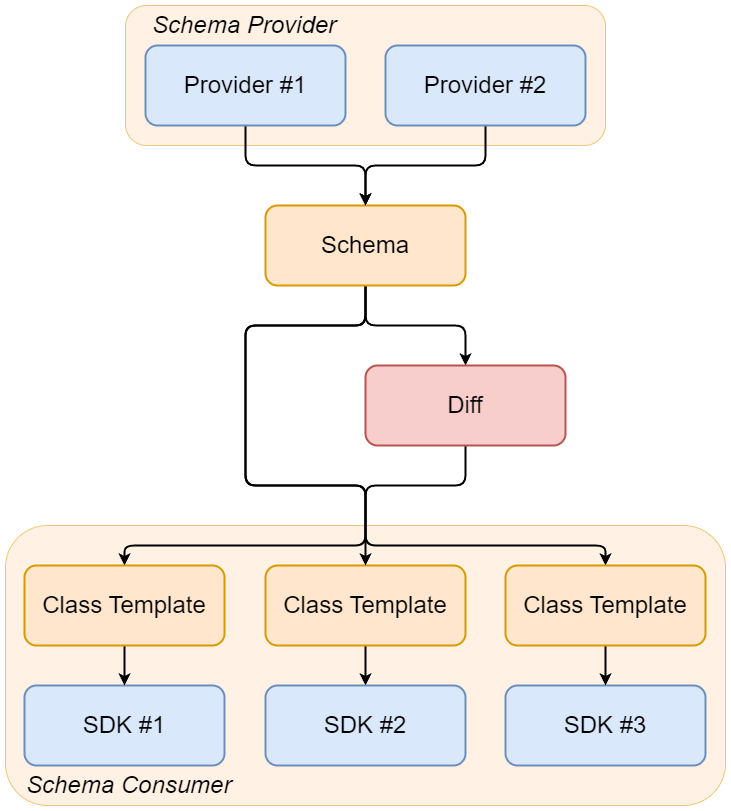
\includegraphics[height=10cm]{figures/assets/mapping_flow.png}
    \caption{Flow of entire solution}
    \label{fig:mapping_flow}
\end{figure}


\subsection{Creating a schema definition \label{sec:design:scema_definiton}}
The backbone of the entire prototype is the schema. 
DTOs will be converted into schemas, and SDKs will created from schemas.
The purpose of this schema is to define the structure of the DTO, and potentially act as the single source of truth.
While iterating over the design, the schema has changed format multiple times. 
Each of these designs will be referred to as a phase. 
Before the final schema definition is explained, the phases leading to the final definition are explained.
\begin{itemize}
    \item \textbf{Phase 1: File format}: The decision of the file format. The two proposed formats are YAML and JSON. As YAML is both more human readable, and a superset of JSON \cite{yaml_definiton}, this format was chosen, while still leaving the option for users to use JSON, if wanted.
    \item \textbf{Phase 2: List vs Map}: When defining the models, this phase went back and forth between whether the models should be in a list, with each model as an entry, or in a key-value map, with the key being the unique identifier of the object. This key would often be \( \{namespace\}.\{className\} \), however, this will not be a requirement. A key-value approach is chosen here, based on mainly two reasons; it is easier for humans to quickly see what type it is, and by taking inspiration from OpenAPI.
    \item \textbf{Phase 3: Additional properties}: When exploring hierarchy, it was identified the original definition was lacking properties necessary to implement this. To solve this, additional optional properties were added to the definition. If these properties are not needed, the schema can omit them.
    \item \textbf{Phase 4: Schema Type}: When exploring enums, it was identified that a single format for schemas is insufficient, as a class an enum is different, and thereby needs different properties. Therefore, a required property called \textit{type} was introduced, specifying if it is a class or an enum schema, and a new enum schema was created.
    \item \textbf{Phase 5: Generics}: Like in phase 3, new properties were needed when adding generics, however, this is not all that is required here. When defining a type, it is until now guaranteed to be a valid class. However, with the addition of generics, the type can now be either a generic \textit{T} or a type with a generic type, e.g. \textit{List\textless T\textgreater} or \textit{List\textless string\textgreater}. For classes, an additional optional property was added. For class properties, the same syntax as both C\#, Java, TypeScript, and other languages was used, meaning the value will be written the same as was just showcased. This means the Schema Consumer will be able to check if the type contains a \textless to indicate if it is a generic. Furthermore, it will be possible to detect if it is a class generic argument, or an implementation, by matching the type with the generic types that are defined in the class.
\end{itemize}
\noindent
By undergoing all of these phases, the final design is ready. The definition itself can viewed in Table \ref{tab:schame_exmaple_final}. For a better understanding of the definition, an example is further included in Listing \ref{code:schame_exmaple_final}. Furthermore, previous definitions are included in appendix \ref{appendix:schemas}, to showcase the design journey.
\begin{table}[H]
   \small
   \centering
   \begin{ctabularx}{\textwidth}{llX}
   
   \toprule
   \multicolumn{3}{l}{\textbf{Schema Structure}} \\
   \midrule
   \textit{Field} & \textit{Type} & \textit{Description} \\ 
   \midrule
   type & string & The type of the schema, either \textit{object} or \textit{enum} \\
   namespace & string & Which namespace the class belongs to \\
   name & string & The name of the class \\

   \midrule
   \multicolumn{3}{l}{\textbf{Object Schema Structure : Schema Structure}} \\
   \midrule
   \textit{Field} & \textit{Type} & \textit{Description} \\ 
   \midrule
   abstract? & boolean & If the class is an abstract class \\
   extends? & string & Which class the class extends \\
   generics & string[] & A list of all the generic values the class contains \\
   properties & Property[] & A list of all the properties the class contains \\

   \midrule
   \multicolumn{3}{l}{\textbf{Enum Schema Structure : Schema Structure}} \\
   \midrule
   \textit{Field} & \textit{Type} & \textit{Description} \\ 
   \midrule
   values & string[] & A list of all the enum values \\
   
   \midrule
   \multicolumn{3}{l}{\textbf{Property Structure}} \\
   \midrule
   \textit{Field} & \textit{Type} & \textit{Description} \\ 
   \midrule
   type & string & The type of the property, either a built-in type, or the key in the schema map. \\
   name & string & The name of the property \\
   nullable & boolean & If the property is marked as nullable \\
   \bottomrule
   \end{ctabularx}
   \caption{Schema definiton} 
   \label{tab:schame_exmaple_final}
\end{table}

\begin{lstlisting}[caption={Schema definition}, label={code:schame_exmaple_final}, style=yaml]
schemas:
  "SchemaExtractor.Model.Example.Person":
    type: "object"
    namespace: "SchemaExtractor.Model.Example"
    name: "Person"
    generics:
    - "T"
    properties:
    - type: "string"
      name: "Name"
      nullable: false
    - type: "SchemaExtractor.Model.Example.Gender"
      name: "Gender"
      nullable: false
    - type: "T"
      name: "GenericProp"
      nullable: true
    - type: "List<SchemaExtractor.Model.Example.Person<T>>"
      name: "Parents"
      nullable: false
    - type: "Map<string, SchemaExtractor.Model.Example.Address>"
      name: "Address"
      nullable: false
  "SchemaExtractor.Model.Example.Gender":
    type: "enum"
    namespace: "SchemaExtractor.Model.Example"
    name: "Gender"
    values:
    - "Male"
    - "Female"
  "SchemaExtractor.Model.Example.Address":
    type: "object"
    namespace: "SchemaExtractor.Model.Example"
    name: "Address"
    properties:
    - type: "string"
      name: "Street"
      nullable: false
    - type: "int32"
      name: "Number"
      nullable: false
\end{lstlisting}

\subsubsection{Adding support for native built-in types}
By deep diving into Listing \ref{code:schame_exmaple_final}, it shows some types does not define a full path, such as string and int32.
This is due to the schema having some ''\textit{built-in-types}''. These are types that are not defined as schemas, but instead a native part, which a Schema Consumer should be able to consume. Table \ref{tab:built_in_types} lists all the built-in types. If a property uses a type that is not defined here, it should be defined as its own schema.

\begin{table}[H]
   \small
   \centering
   \begin{ctabularx}{\textwidth}{lX}
   
   \toprule
   Type & Description \\
   \midrule
   boolean & A boolean input \\
   int32 & A 32-bit signed integer \\
   int64 & A 64-bit signed integer \\
   float & A 32-bit floating point \\
   double & A 64-bit floating point \\
   char & Represent a single character \\
   string & A collection of characters, as a single string. \\
   object & A wildcard type. This type has not explicitly been stated, and everything should be accepted. \\
   guid & A GUID / UUID \\
   date & A date, that includes both date and time \\
   dateOnly & A date, that only specifies the date and not the time \\
   dateTimeOffset & A date, that includes both date, time, and time offset \\
   List & A list of items. \\
   Map & A key-value pair. Often referred to as either a map or dictionary in code. \\
   \bottomrule
   \end{ctabularx}
   \caption{Built In Types} 
   \label{tab:built_in_types}
\end{table}

\subsubsection{Adding support for generics}
The adaptation of generics has a significant impact on the schema definition.
The major decision is between should the schema be updated with new fields, or should the generics be added to the current schema, and have a custom parser.
The later option is chosen, where a property type is defined the same was, as both \textit{C\#}, \textit{Java} and \textit{TypeScript}. To change e.g. a \textit{string} type, to a generic string list, the type is updated to \textit{List\textless string\textgreater}. When parsing a type, there should therefore be checked for \textit{\textless}, and if found, the type should be parsed as a generic type.
A pseudo implementation is suggested in Algorithm \ref{alog:parse_type}
\begin{algorithm}
\caption{Parse Type}
\label{alog:parse_type}
\begin{algorithmic}[1]

\Function{parseType}{type}
    \State genericStart $\gets$ indexOf(type, "\textless")
    \If{genericStart == -1}
        \State \textbf{return} type
    \EndIf

    \State splitType $\gets$ split(type, genericStart)
    \State genericType $\gets$ splitType[0]
    \State genericImpl $\gets$ parseType(substring(splitType[1], 0, length(splitType[1]) - 1))
    \State \textbf{return} combine(genericType, genericImpl)
\EndFunction
\end{algorithmic}
\end{algorithm}

\subsection{Designing a schema provider \label{sec:design:schema_provider}}
By having understood the schema, the Schema Provider can now be designed. The purpose of this is to take an existing solution and convert all DTOs defined here into schemas. This will enable the solution to act as a single source of truth for all DTOs.
It is possible to create multiple schema providers if the code base is scattered across multiple languages.
\newline\newline
The schema provider works by taking a single DTO, and from that output all necessary schemas. 
The reason why a single DTO can output multiple schemas is that both derived classes and classes used in properties should be defined. This is a recursive process, where the same steps are performed for all property types and derived types.
An example of this is showcased in Figure \ref{fig:schema_provider_flow}, where a single DTO outputs five different schemas. 
These generated schemas would be:
\begin{itemize}
    \item The own class itself
    \item The class it derives from, in this example called \textit{ParentClass}
    \item All the classes used in the properties of the class, in this example \textit{ClassOne}, \textit{ClassTwo} and \textit{ClassThree}
\end{itemize}

\begin{algorithm}
\caption{Pseudo code for converting a DTO to a schema}
\label{code:schema_provider_pseudo}
\begin{algorithmic}[1]

\State allSchemas $\gets$ []

\Function{convertClass}{type}
    \If{type is in allSchemas}
        \State \textbf{return}
    \EndIf

    \State allSchemas.add(generateSchema(type))

    \If{type.isDerived}
        \State convertClass(type.parentType)
    \EndIf

    \For{each property in type.properties}
        \State convertClass(property.type)
    \EndFor
\EndFunction

\end{algorithmic}
\end{algorithm}

\begin{figure}[h!]
    \centering
    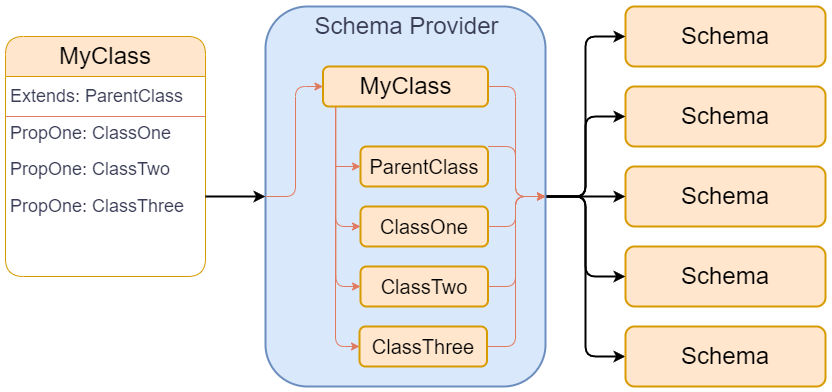
\includegraphics[width=\textwidth]{figures/assets/schema_provider_flow.png}
    \caption{Schema Provider flow}
    \label{fig:schema_provider_flow}
\end{figure}


\subsection{Designing a schema consumer \label{sec:design:schema_consumer}}
To create the final SDKs, the specified schemas should be consumed, an transformed into code.
As showcased in Figure \ref{fig:mapping_flow}, a single schema can be turned into multiple templates, and thereby into a class in an SDK.
The individual journey for creating a single SDK is illustrated in Figure \ref{fig:schema_consumer_flow}, and will be looped for each target language.

\begin{figure}[h!]
    \centering
    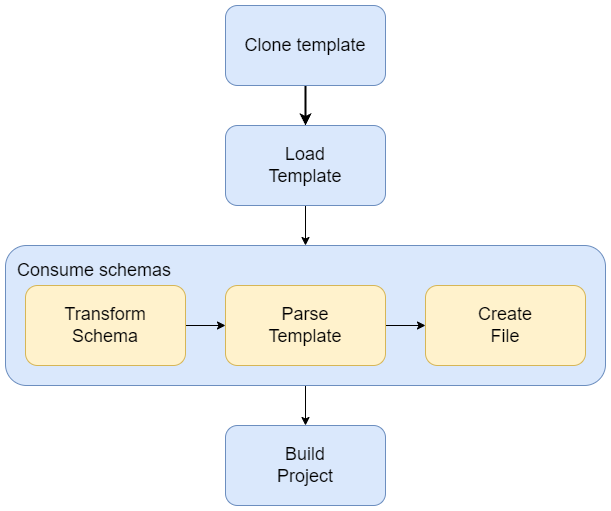
\includegraphics[width=12cm]{figures/assets/schema_consumer_flow.png}
    \caption{Schema Consumer flow}
    \label{fig:schema_consumer_flow}
\end{figure}

\noindent
Furthermore, the steps are explained in detail here.
\begin{itemize}
    \item \textbf{Clone template}: The target language template is cloned to the output. What is included in this template, will be explored in Section \ref{sec:design:default_projects}.
    \item \textbf{Load template}: The class template for the target language is loaded and parsed, allowing for quick placeholder replacement.
    \item \textbf{Consume schemas}: The following steps will be executed for each schema that should be converted.
    \begin{itemize}
        \item \textbf{Transform schema}: The schema is transformed to a language-specific data container, allowing for custom parsing of data, e.g. properties.
        \item \textbf{Parse template}: The class template is parsed with the data, resulting in a complete class.
        \item \textbf{Create file}: The class is written to a file, with a file type associated with the language.
    \end{itemize}
    \item \textbf{Build project}: The project is built, using the language-specific build tools.
\end{itemize}


\subsubsection{Adding default template projects \label{sec:design:default_projects}}
As specified, it should be possible to clone a default project, as each language has a file structure that needs to be followed. The alternative is to programmatically create files and populate these files with data, however, since the default files remain the same, they are simply cloned instead.
This means that the developer can create a template project via the language's own tools, and build the SDK on top of this. If multiple versions of the same language should be added, the developer can then simply create two templates, one with each version. Furthermore, different package managers, default dependencies, and similar things can be included in this template. This may result in a large number of default projects, but that is by design, as it can cater to everyone's specific needs.


\subsection{Designing a semantic difference checker \label{sec:design:diff_checker}}
The job of the Diff Checker is to find all semantic differences between a list of schemas.
This can be done by taking all the schemes and removing the shared schemas, as shown in equation \ref{equation:diff_set}.
\begin{equation}
\label{equation:diff_set}
    \Delta = A \bigcup B - A \bigcap B
\end{equation}
\noindent
An example of this is shown in Figure \ref{fig:diff_checker}, which shows two lists, and old list \textit{A}, and a new list \textit{B}.
\begin{figure}[h ]
    \centering
    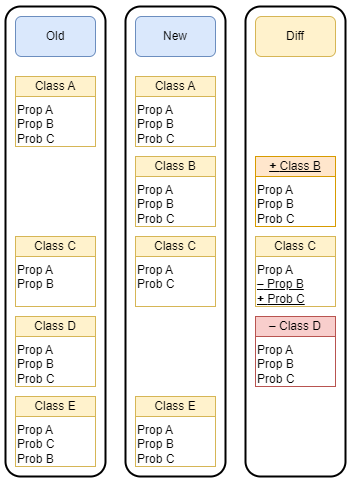
\includegraphics[height=12cm]{figures/assets/diff_checker.png}
    \caption{Diff checker result}
    \label{fig:diff_checker}
\end{figure}
\noindent
The Diff Checker will compare the figures semantically, meaning the order of properties does not matter, as long as all properties are included.
\begin{itemize}
    \item \textbf{Class A}: Two identical classes, and therefore there is no difference.
    \item \textbf{Class B}: A new class that has been added
    \item \textbf{Class C}: A class where a property has been removed, and replaced with another
    \item \textbf{Class D}: A class that has been removed
    \item \textbf{Class E}: A class where the order of properties has been switched, but remains semantically identical, which results in there being no difference.
\end{itemize}
In this case, both \textit{Class C} and \textit{Class D} should give a warning, as these classes have changed. As \textit{Class B} is a new addition, there is no need for a warning, and it can be added. From here, a developer should determine if the changes the Diff Checker warns about are acceptable or not. An acceptable change could be a planned change, where they are aware it is a breaking change. Are the changes accepted, the schemas can be transformed to an SDK, and the schemas the Diff Checker checks against can be updated with the new content.
\section{Implementation \label{sec:implementation}}

\subsection{Schema Provider}
For this prototype, only a single Schema Provider has been implemented, which is a C\# Schema Provider.
This will follow the principles defined in Section \ref{sec:design:schema_provider}.
One of the main features is the mapping of built-in types.
As the definition does not specify a built-in type for all the types provided in C\#, multiple types have been mapped to the same built-in type.
An example of this is \textit{byte}, \textit{short} and \textit{int} all being mapped to a \textit{int32}.
A full example of how types are mapped can be viewed in Listing \ref{lst:dto_type_provider}, where the mapping to \textit{int32} is highlighted. 
\begin{lstlisting}[caption={C\# type schema mapping}, label={lst:dto_type_provider}, style=base_csharp]
dtoDirectory
    .AddMapping<bool>("boolean")
    .AddMapping<char>("char")
    .AddMapping<string>("string")
     // ------------
    .AddMapping<byte>("int32")
    .AddMapping<sbyte>("int32")
    .AddMapping<short>("int32")
    .AddMapping<ushort>("int32") 
    .AddMapping<decimal>("int32")
    .AddMapping<int>("int32")
    .AddMapping<uint>("int32")
    .AddMapping<nint>("int32")
    .AddMapping<nuint>("int32")
     // ------------
    .AddMapping<long>("int64")
    .AddMapping<ulong>("int64")
    .AddMapping<float>("float")
    .AddMapping<double>("double")
    .AddMapping<Guid>("guid")
    .AddMapping<DateOnly>("dateOnly")
    .AddMapping<DateTime>("date")
    .AddMapping<DateTimeOffset>("dateTimeOffset")
    .AddMapping(typeof(List<>), "List")
    .AddMapping(typeof(HashSet<>), "List")
    .AddMapping(typeof(Dictionary<object, object>), "Map");
\end{lstlisting}
\noindent
Other than the mapping, the implementation does not have anything special, that is not discussed in section \ref{sec:design:schema_provider}.
The program converts on class to a schema at a time and adds it to an internal storage.
Afterwards, all associated classes are converted the same way.
All the mapping is done according to the specification of the schema, with properties either being a built-in type, as mapped in Listing \ref{lst:dto_type_provider}, or another schema.
Once all classes have been mapped, the list of all schemes can be extracted from the storage, in serialized.

\subsection{Schema Consumer}
The schema consumer is designed to allow adding multiple languages with minimum code.
By limiting the unique amount of work required for each language to be implemented, the support is easily
This is done by handling as much as the transformation behind the scenes, and only having a few interfaces that would need to be implemented to add support for a new language.

\subsubsection{Built in types \label{sec:implementation:built_in_types}}
To accommodate built-in types having different formats in different programming languages, it is possible to register custom converters. Listing \ref{lst:dto_type_consumer} shows how all built-in types are registered.
\begin{lstlisting}[caption={Schema types to C\# mapping}, label={lst:dto_type_consumer}, style=base_csharp]
dtoDirectory
    .Register<object>("object")
    .Register<bool>("boolean")
    .Register<char>("char")
    .Register<string>("string")
    .Register<int>("int32")
    .Register<long>("int64")
    .Register<float>("float")
    .Register<double>("double")
    .Register<Guid>("guid")
    .Register<DateOnly>("dateOnly")
    .Register<DateTime>("date")
    .Register<DateTimeOffset>("dateTimeOffset")
    .Register(typeof(List<>), "List")
    .Register(typeof(Dictionary<object, object>), "Map");
\end{lstlisting}
All registered types require a custom Type Converter, which is shown in Listing \ref{lst:ITypeConvertor}.
\begin{lstlisting}[caption={ITypeConvertor interface}, label={lst:ITypeConvertor}, style=base_csharp]
public interface ITypeConvertor<T> : ITypeConvertor
{
    Type ITypeConvertor.TypeToConvert() => typeof(T);
    public string ConvertProperty(SchemaProperty context);
}
\end{lstlisting}
\noindent
The implementation of the type converter, tells the system how to format a property for the target language.
An example of the need for this interface is when e.g. converting an \textit{int32}. In Java, the property type would be \textit{int}, while it would be \textit{number} in TypeScript.

\subsubsection{Class Converter}
Another one of the main features of the solution is the implementations of the \textit{IClassConverter} interface, which can be seen in Listing \ref{lst:class_converter}.
This class serves as the main element to convert a schema to a complete SDK.

\begin{lstlisting}[caption={IClassConvertor interface}, label={lst:class_converter}, style=base_csharp]
public interface IConvertor
{
    public string TargetLanguage { get; }
}

public interface IClassConvertor : IConvertor
{
    /// <summary>
    /// Defines the template from which a class template is created from.
    /// Placeholders, conditions and more are supported via <see href="https://github.com/scriban/scriban">Scriban</see>.
    /// </summary>
    /// <returns>A complete class template.</returns>
    public string GetClassTemplate();

    /// <summary>
    /// Formats a class property, to be ready to add into the class.
    /// The output will be available when parsing the class template.
    /// </summary>
    /// <param name="classProperty">The details for the property.</param>
    /// <returns>A formatted property.</returns>
    public string FormatProperty(ClassProperty classProperty);

    /// <summary>
    /// An optional way to further transform a class template, after the system has performed the initial transformation.
    /// </summary>
    /// <param name="classTemplate">The pre parsed template</param>
    /// <returns>An updated template</returns>
    public ClassTemplate PostTransform(ClassTemplate classTemplate)
    {
        return classTemplate;
    }
}
\end{lstlisting}
\noindent
To better understand how this interface is used, an in-depth explanation, with examples, is provided.
The main functionality lies in the following three methods.
\begin{itemize}
    \item \textbf{GetClassTemplate}: This provides a class template, that when populated will create an entire class for the specific language.
    This is the one of the core functions that drives the entire solution.
    The code in Listing \ref{lst:java_class_converter_getclasstemplate} shows an example of a Java class.
    \begin{lstlisting}[caption={Implementation of a Java class template}, label={lst:java_class_converter_getclasstemplate}, style=base_csharp]
    package {{namespace}};
    
    import {{import}};
    
    public class {{class}} {
        
        {{property}};
    
        
        {{method}};
    
    }
    \end{lstlisting}

    \item \textbf{FormatProperty}: Instead of having the class template containing checks properties, a separate method is instead used to parse these properties.
    This should return a correctly formatted property, which can be directly inserted into the class template.
    Listing \ref{lst:java_class_converter_formatproperty} shows an example on how Java properties are formatted.
    \begin{lstlisting}[caption={How a Java property is defined}, label={lst:java_class_converter_formatproperty}, style=base]
$"{(classProperty.Nullable ? "@Nullable" : "@NotNull")}\n\t" +
$"private {classProperty.Type} {classProperty.Name};";
    \end{lstlisting}
    \noindent

    \item \textbf{PostTransform}: The last method is an optional way to transform the Class Template further than is done behind the scenes, and create custom data for the specific language.
    This is e.g.\ used in Java to create getters, which is not needed in either TypeScript or C\#.
\end{itemize}

\subsection{Diff Checker}
When implementing the Difference Checker, a Diff Schema is needed. 
The purpose of this schema is to return all changes to the user. 
The checker will iterate over all schemes, returning a list of all changes.
It will differentiate objects by the key of the schema. This means, that if a key name has been modified, the system will treat it as if the old schema has been removed, and a new one has been added.
A full example of how the diff schema is defined can be viewed in Listing \ref{code:diff_example}.
\begin{lstlisting}[caption={Diff schema example}, label={code:diff_example}, style=yaml]
- type: "Removed"
  namespace: "Example.Model"
  name: "TestClass01"
- type: "Added"
  namespace: "Example.Model"
  name: "TestClass02"
- type: "Modified"
  namespace: "Example.Model"
  name: "TestClass03"
  differences:
    - path: "abstract"
      oldValue: "false"
      newValue: "true"
    - path: "generics"
      oldValue: "[TKey, TValue]"
      newValue: "[TKey, TVValue, TDefault]"
  properties:
    - type: "Removed"
      name: "MyProp1"
    - type: "Added"
      name: "MyProp2"
    - type: "Modified"
      name: "MyProp3"
      differences:
        - path: "type"
          oldValue: "string"
          newValue: "int32"
        - path: "nullable"
          oldValue: "true"
          newValue: "false"
\end{lstlisting}
\section{Evalutaion}

\subsection{An overview of the DTOs used to evaluate the prototype}
To properly evaluate the prototype, an advanced DTO structure has been created. It involves a complex and nested structure.
The example DTOs consist of 486 properties, across 93 different classes.
Based on the results found in the analysis, it can be estimated that a manual conversion would take approximately 2 hours and 42 minutes, as seen in Equation \ref{equation:time_saved_example}.
\begin{equation}
\label{equation:time_saved_example}
    486 \text{ properties} \times 20,07 \text{ seconds/properties} = 2h\ 42m\ 34s
\end{equation}
The example DTOs will be used in the data used in the entire evaluation and can be viewed in the source code, available from Appendix \ref{appendix:source_code}

\subsection{Performance Evaluation \label{sec:evaluation:performence_evaluation}}
From the analysis, manual DTO conversion was shown to take an average of 20.07 seconds per property, as documented in Table \ref{tab:dto_task}. This process is labor-intensive and prone to human errors, such as incorrect casing, syntax issues, and nullability errors. 
In contrast, the automated solution provided by the prototype performed these conversions almost instantaneously. 
Table \ref{tab:prototype_time_eval} shows the time it takes for each service to perform its respective task. The time showed, is without any overhead, such as saving the schema as a YAML file or loading schemas from a YAML file.

\begin{table}[h]
    \centering
    \begin{tabular}{lr}
    \toprule
         Service & Time taken \\
    \midrule
         Schema Provider & 21ms \\
         Schema Consumer & 150ms \\
         Diff Checker & 10ms \\
    \bottomrule
    \end{tabular}
    \caption{Prototype time evaluation}
    \label{tab:prototype_time_eval}
\end{table}
\noindent
The total time for running the Schema Provider, validating the schemas with the Diff Checker, and creating a new SDK is \textit{181 ms}, which is insignificant, when compared to the time a manual conversion would take, as shown in Equation \ref{equation:time_saved_example}.
The task that takes the longest time, is consuming the schemas, and creating an SDK. This is mainly due to the I/O operations, where a file is created and written to, for each class generated.
In scenarios where the Diff Checker checks all schemas, and validates there are no changes, this step could be omitted.
\newline\newline
The other major element of the prototype is to reduce the number of errors in the final SDK.
The number of errors is tightly coupled with the implementation of the interfaces. If there are any errors in the supplied interfaces, the error will persist in every class. However, with a correct implementation, all errors are completely eradicated.
For the prototype, the one error that remains is the system uses an invalid casing,
This id due to the casing is extracted from the C\# code, and directly used in the templates.
An implementation of a casing converter, as described by the requirements, would solve this issue.

\subsection{Strengths and Limitations}
The are both strengths and limitations to the developed prototype.
\subsubsection*{Strengths}
\begin{itemize}
    \item \textbf{Efficiency}: As proven by table \ref{tab:prototype_time_eval}, the prototype improves the efficiency of a developer, allowing them to create multiple SDKs at once, and freeing up time to focus on more complex and higher-value tasks, than a time-consuming conversion.
    \item \textbf{Accuracy}: The prototype eliminates all possibility of manual errors. Furthermore, it enforces the same conversions in the entire SDK, as the same rules are followed for every file.
    \item \textbf{Scalability}: The prototype can easily handle complex schemas and large-scale projects, making the prototype suitable for large-scale enterprise solutions.
\end{itemize}

\subsubsection*{Limitations}
\begin{itemize}
    \item \textbf{Initial Setup}: While a lot of time and errors can be saved, it may be a time-consuming task to set up the prototype for a project. This may prevent small projects from utilizing the prototype, as the time it takes to implement, may be greater than the time a manual conversion will take.
    \item \textbf{Customization}: The prototype has no configuration at all, and is therefor not suitable for a real-life scenario.
    \item \textbf{Evaluation Scope}: The prototype has not been validated and tested by stakeholders, or in any real-life scenario, but is instead developed from a theoretical aspect, and tested with theoretical cases. 
\end{itemize}

\subsection{Fulfillment of requirements}
The prototype has not implemented all requirements, as defined in the requirements in Table \ref{tab:requirements}. Instead, only the bare-bone required requirements has been implemented. The status of all implemented requirements can be viewed in Table \ref{tab:fulfilled_requirements}.
\begin{table}[H]
   \small
   \centering
   \begin{ctabularx}{\textwidth}{llX}
   \toprule
   \textit{\#} & \textit{Fulfilled} & \textit{Description} \\ 
   \midrule
   \textbf{1} & Yes & Requirement 1, and all sub-requirements have been fulfilled. \\
   \textbf{2} & Yes & Requirement 2, and all sub-requirements have been fulfilled. \\
   \textbf{3} & Partly & Requirement 3.1 has not been fulfilled. \newline All other sub-requirements have been fulfilled. \\
   \textbf{4} & Yes & Requirement 4, and all sub-requirements have been fulfilled. \\
   \textbf{5} & No & Requirement 5 has not been implemented. \\
   \textbf{6} & No & Requirement 6 has not been implemented. \\
   \textbf{7} & Yes & Requirement 7, and all sub-requirements have been fulfilled. \\
   \bottomrule
   \end{ctabularx}
   \caption{Fufillment of the requirements} 
   \label{tab:fulfilled_requirements}
\end{table}

\section{Future Work}
As described earlier, the implemented solution is a primitive prototype, that acts as a proof of concept. This prototype would not be sufficient in a production environment, due to limited implementation and lack of features. This section will try to go through the steps needed, for the proposed solution to be effective in a real-life scenario.
\subsection{Validation with costumers}
As the project is not fully complete, it has not been verified with customers on their solutions.
That said, the prototype is fully functional and ready to be presented to the stakeholders, but the final product is not ready for production, as several key elements that take it from a prototype to an integrated ready product are missing. Several of these missing parts will be discussed in this section.


\subsection{Implementation of additional features}
\subsubsection*{Adding configuration}
One of the major features missing is the ability to configure the solution.
It is impossible to create a single solution, that would please all developers out of the box. It is therefore important to be able to configure the solution.
An analysis of which setting should be in a production-ready environment has not been made. However, a few settings are suggested.
Some settings are relevant, no matter what the target language is.
\begin{itemize}
    \item \textbf{Property Naming Attribute}: Should the system add an explicit attribute to properties, stating the name of the property in a JSON scheme? 
    \item \textbf{Property Naming Policy}: If the user does not provide a property name attribute, what naming policy should the system default to? 
    \begin{itemize}
        \item \textbf{Camel case}: Name the properties as \textit{camelCase}.
        \item \textbf{Snake case}: Name the properties as \textit{snake\_case}.
        \item \textbf{Pascal case}: Name the properties as \textit{PascalCase}.
        \item \textbf{None}: Do not modify the property name in any way.
    \end{itemize}
    \item \textbf{Output directory}: Where should the outputted SDK be created?
\end{itemize}
\noindent
On top of the general options, some options are specific for each individual language.
\begin{itemize}
    \item \textbf{Java: Root Package}: In Java, namespaces often has a root, often a domain the user owns. This setting indicates what, if anything, should be prepended to the namespace.
    \item \textbf{Property Naming Policy}: If the user does not provide a property name attribute, what naming policy should the system default to? 
    \item \textbf{Output directory}: Where should the outputted SDK be created?
    
\end{itemize}


\subsubsection*{Add options to change used 3rd party libraries}
It should be possible to customize which libraries the generated SDK includes.
This is potentially already possible, as it is possible to create multiple default projects, that are cloned. A new version could be created, where other default libraries are installed, resulting in the final SDK having those included.
For the default projects that are included with the solution, they must include as few as possible libraries, to reduce both the size of the generated SDK and the libraries it will provide when added to a project.

\subsubsection*{Schema naming convention}
At the moment, there is not defined any standard for how a class or property should be named.
What is input in the schema, will be what is created in each SDK.
However, languages often have different naming conventions they follow.
An example of this is Java using \textit{camelCase}, C\# using \textit{PascalCase} and Python using \textit{snake\_case}.
Therefore, there should be defined a naming convention, and each language map to follow the language-specific style.


\subsubsection*{Add support for custom serilizers}
When creating the Schema Provider, it should be possible to create custom sterilizer for data.
It could be that the internal code handles a type as numbers, but the API exposes them as strings, or having a class being on encapsulation if a property, where the API only provides the encapsulated property. This should be implemented similarly to the ITypeConverter defined in section \ref{sec:implementation:built_in_types}, with a different name, possible \textit{ITypeSerilizer}


\subsection{Expanding with an auto-generated HTTP client}
As one of the major use cases of DTOs is HTTP communication, a suggested addition to the solution is an auto-generated HTTP client. 
When analysing a code-space in the Schema Provider, it could further scan the same codespace if any HTTP endpoints have been defined, and include this information in the schema.
The inclusion of an HTTP client would further benefit the use of the SDK, as neither the developers or users would need to manually built this on top of the generated SDK.
This also refers back to the example showcased in both Listing \ref{code:http_example_csahrp} and Listing \ref{code:http_example_typescipt}, where the need for automated SDKs were introduced.
To implement this HTTP client an update to the schemas is required, to allow for endpoints to be defined. An early design of this is shown in Listing \ref{code:http_client_schema}.
\begin{lstlisting}[caption={Example of adding endpoints to the schema definition}, label={code:http_client_schema}, style=yaml]
endpoints:
  # Base URL
  "localhost:3000":
    - path: "api/users/{userId}"
      method: "GET"
      parameters:
        userId: "string"
      response: "SchemaExtractor.Model.Example.Person"
    - path: "api/users"
      method: "POST"
      body: SchemaExtractor.Model.Example.CreatePersonDto
      response: "SchemaExtractor.Model.Example.Person"
schemas: {...}
\end{lstlisting}
Furthermore, the Diff Checker should be included in this updated schema. By both validating schemas and endpoints, there is further protection against unintentional changes.


\subsection{Continuous Integration}
To maximize the benefits of the Semantic Versioned SDK Generation prototype, it is necessary to integrate it into a continuous integration (CI) pipeline. Having the prototype included within CI processes has several notable advantages:

\begin{itemize}
    \item \textbf{Automated SDK Generation} Incorporating this prototype in a CI pipeline would automatically generate SDKs whenever there are changes. This means that they will always be up-to-date with the latest coding changes, which eliminates the possibility of mismatch between source code and SDKs.
    
    \item \textbf{Automated Testing and Validation} Integration of CI automates validation for produced SDKs. This makes sure that errors or inconsistencies are not introduced when changing DTOs or schema. Any breaking changes can be instantly found. Therefore, this continuous process ensures high-quality code
\end{itemize}

\section{Conclusion}
This paper set out to validate the hypothesis, that an automated SDK generation could save both time and reduce errors. 
To validate the hypothesis, the time it takes a developer, and the amount of bugs is created in the process are compared with the automated prototype.
\begin{itemize}
    \item \textbf{Time Savings}: The prototype shows a clear indication that the potential time saving is quite significant. It goes from approximately 2 hours and 40 minutes to shy of 200 microseconds to create the same SDK.
    \item \textbf{Error Reduction}: The reduction of errors is not as proven, as the time savings, This is mainly due to the limitations of the SDK. As described in Section \ref{sec:evaluation:performence_evaluation}, the prototype is shipped with known casing bugs. However, with further development, the rate of bugs can be greatly reduced. Furthermore, once a bug is addressed in the prototype, it will be permanently fixed, and not occur again.
\end{itemize}
\noindent
As the sub-hypothesis has been validated, the main hypothesis is also validated.


\DeclareFieldFormat{urldate}{
  \textit{(visited on: \thefield{urlday}/\thefield{urlmonth}/\thefield{urlyear})}
} %% Set the last visited on text to DD-MM-YYYY
\printbibliography[heading=bibintoc,]

\newpage
\begin{appendices}
\usepackage{listings}

\lstdefinestyle{base} {
  aboveskip=3mm,
  belowskip=3mm,
  showstringspaces=false,
  columns=flexible,
  basicstyle={\small\ttfamily},
  numbers=none,
  numberstyle=\tiny\color{gray},
  keywordstyle=\color{blue},
  commentstyle=\color{dkgreen},
  stringstyle=\color{string},
  breaklines=true,
  breakatwhitespace=true,
  tabsize=3,
  numbers=left,
  stepnumber=1,
}

% CSharp
\lstdefinestyle{base_csharp} {%
  language=[Sharp]C, 
  morekeywords={nint, unit, nuint, var, await},
  style=base
}
\lstnewenvironment{csharp}{%
    \lstset{%
        style=base_csharp,
    }
}{}


% Java
\lstdefinestyle{base_java} {%
  language=Java, 
  style=base
}

\lstnewenvironment{java}{%
    \lstset{%
        style=base_java,
    }
}{}

% Typescript
\lstdefinestyle{base_typescript} {
  style=base,
  keywords={abstract, any, as, boolean, break, case, catch, class, console, 
    const, continue, debugger, declare, default, delete, do, else, enum, export, 
    extends, false, finally, for, from, function, get, if, implements, import, in, 
    infer, instanceof, interface, keyof, let, module, namespace, never, new, null, 
    number, object, package, private, protected, public, readonly, require, return, 
    set, static, string, super, switch, symbol, this, throw, true, try, type, typeof, await,
    undefined, unique, unknown, var, void, while, with, yield},
  morecomment=[s]{/*}{*/},
  morestring=[b]',
  morestring=[b]",
  morestring=[b]`,
  sensitive=true
}

\lstnewenvironment{typescript}{%
    \lstset{%
        style=base_typescript,
    }
}{}

\lstdefinestyle{yaml} {
  style=base,
  keywords={true,false,null,y,n},
  comment=[l]{\#},
  morestring=[b]',
  morestring=[b]",
  sensitive=true
}
\section{Schema definitions \label{appendix:schemas}}
\begin{table}[H]
   \small
   \centering
   \begin{ctabularx}{\textwidth}{llX}
   
   \toprule
   \multicolumn{3}{l}{\textbf{Schema Structure extends Schema Structure}} \\
   \midrule
   \textit{Field} & \textit{Type} & \textit{Description} \\ 
   \midrule
   type & string & The type of the schema, either \textit{object} or \textit{enum} \\
   namespace & string & Which namespace the class belongs to \\
   name & string & The name of the class \\

   \midrule
   \multicolumn{3}{l}{\textbf{Object Schema Structure extends Schema Structure}} \\
   \midrule
   \textit{Field} & \textit{Type} & \textit{Description} \\ 
   \midrule
   abstract? & boolean & If the class is an abstract class \\
   extends? & string & Which class the class extends \\
   properties & Property[] & A list of all the properties the class contains \\

   \midrule
   \multicolumn{3}{l}{\textbf{Enum Schema Structure extends Schema Structure}} \\
   \midrule
   \textit{Field} & \textit{Type} & \textit{Description} \\ 
   \midrule
   values & string[] & A list of all the enum values \\
   
   \midrule
   \multicolumn{3}{l}{\textbf{Property Structure}} \\
   \midrule
   \textit{Field} & \textit{Type} & \textit{Description} \\ 
   \midrule
   type & string & The full name of the type, both namespace and class combined \\
   name & string & The name of the property \\
   nullable & boolean & If the property is marked as nullable \\
   \bottomrule
   \end{ctabularx}
   \caption{Thrid iteration of the schema} 
   \label{tab:schame_exmaple_three}
\end{table}
\begin{lstlisting}[caption={Thrid iteration of the schema}, label={code:schame_exmaple_three}, style=yaml]
schemas:
  - type: "object"
    namespace: "SdkGenerator.Model.Example"
    name: "LivingEntity"
    abstract: true
    properties:
      - type: "int32"
        name: "age"
        nullable: false
  - type: "object"
    namespace: "SdkGenerator.Model.Example"
    name: "Person"
    extends: "SdkGenerator.Model.Example.LivingEntity"
    properties:
      - type: "string"
        name: "firstname"
        nullable: false
  - type: "enum"
    namespace: "SdkGenerator.Model.Example"
    name: "MyEnum"
    values:
      - "ValueOne"
      - "ValueTwo"
      - "ValueThree"
\end{lstlisting}


\begin{table}[H]
   \small
   \centering
   \begin{ctabularx}{\textwidth}{llX}
   \toprule
   \multicolumn{3}{l}{\textbf{Schema Structure}} \\
   \midrule
   \textit{Field} & \textit{Type} & \textit{Description} \\ 
   \midrule
   namespace & string & Which namespace the class belongs to \\
   name & string & The name of the class \\
   abstract? & boolean & If the class is an abstract class \\
   extends? & string & Which class the class extends \\
   properties & Property[] & A list of all the properties the class contains \\
   \midrule
   \multicolumn{3}{l}{\textbf{Property Structure}} \\
   \midrule
   \textit{Field} & \textit{Type} & \textit{Description} \\ 
   \midrule
   type & string & The full name of the type, both namespace and class combined \\
   name & string & The name of the property \\
   nullable & boolean & If the property is marked as nullable \\
   \bottomrule
   \end{ctabularx}
   \caption{Second iteration of the schema} 
   \label{tab:schame_exmaple_two}
\end{table}
\begin{lstlisting}[caption={Second iteration of the schema}, label={code:schame_exmaple_two}, style=yaml]
schemas:
  - namespace: "SdkGenerator.Model.Example"
    name: "LivingEntity"
    abstract: true
    properties:
      - type: "int32"
        name: "age"
        nullable: false
  - namespace: "SdkGenerator.Model.Example"
    name: "Person"
    extends: "SdkGenerator.Model.Example.LivingEntity"
    properties:
      - type: "string"
        name: "firstname"
        nullable: false
\end{lstlisting}


\begin{table}[H]
   \small
   \centering
   \begin{ctabularx}{\textwidth}{llX}

   \toprule
   \multicolumn{3}{l}{\textbf{Schema Structure}} \\
   \midrule
   \textit{Field} & \textit{Type} & \textit{Description} \\ 
   \midrule
   namespace & string & Which namespace the class belongs to \\
   name & string & The name of the class \\
   properties & Property[] & A list of all the properties the class contains \\
   \midrule
   \multicolumn{3}{l}{\textbf{Property Structure}} \\
   \midrule
   \textit{Field} & \textit{Type} & \textit{Description} \\ 
   \midrule
   type & string & The full name of the type, both namespace and class combined \\
   name & string & The name of the property \\
   \bottomrule
   \end{ctabularx}
   \caption{First iteration of the schema} 
   \label{tab:schame_exmaple_one}
\end{table}

\begin{lstlisting}[caption={First iteration of the schema}, label={code:schame_exmaple_one}, style=yaml]
schemas:
  - namespace: "SdkGenerator.Model.Example"
    name: "LivingEntity"
    properties:
      - type: "int32"
        name: "age"
  - namespace: "SdkGenerator.Model.Example"
    name: "Person"
    properties:
      - type: "string"
        name: "firstname"
\end{lstlisting}

\section{DTO Conversion Guide \label{appendix:convert_guide}}
\subsection{Convert guide for Java}
\begin{lstlisting}[caption={DTO conversion guide for Java}, label={code:convert_guide_java}, style=base]
# How to create DTOs with Java

## Prerequisites
You must have Java and Maven installed.
To validate this, run `mvn -v` and `java -version`

## Step by step guide
1) Check out the project `git clone git@github.com:Arkobat/SdkGenerator.git`
2) Navigate to this folder `cd .\SdkGenerator\Templates\Java\`
3) Create a new branch for your changes `git swtich -c <branch_name>`. Replace `<branch_name>` with something unique, e.g. your GitHub username.
4) Install the dependencies `mvn install`
5) Open the project in your desired IDE, and create the files needed
   - You are free to create both folders and files as pleases you
   - This is an example DTO, you can take inspiration from.
```typescript
package sdk;

import com.google.gson.annotations.SerializedName;
import org.jetbrains.annotations.NotNull;
import org.jetbrains.annotations.Nullable;

public class ExampleDto {

   @NotNull
   @SerializedName("name")
   private String name;

   @SerializedName("version")
   private int version;

   @Nullable
   @SerializedName("childNode")
   private String childNode;

   @Nullable
   @SerializedName("parentNode")
   private String parentNode;


   public @NotNull String getName() {
      return name;
   }

   public int getVersion() {
      return version;
   }

   public @Nullable String getChildNode() {
      return childNode;
   }

   public @Nullable String getParentNode() {
      return parentNode;
   }

}
```
6) Build the project with `mvn package`
7) Commit and push the files `git commit -am "Creates DTOs" && git push`
8) Now you are done
\end{lstlisting}
\subsection{Convert guide for TypeScript}
\begin{lstlisting}[caption={DTO conversion guide for TypeScript}, label={code:convert_guide_typescript}, style=base]
# How to create DTOs with TypeScript

## Prerequisites
You must have NPM installed.
To validate this, run `npm -v`

## Step by step guide
1) Check out the project `git clone git@github.com:Arkobat/SdkGenerator.git`
2) Navigate to this folder `cd .\SdkGenerator\Templates\TypeScript\`
3) Create a new branch for your changes `git swtich -c <branch_name>`. Replace `<branch_name>` with something unique, e.g. your GitHub username.
4) Install the dependencies `npm install`
5) Open the project in your desired IDE, and create the files needed
   - You are free to create both folders and files as pleases you
   - This is an example DTO, you can take inspiration from.
```typescript
export interface ExampleDto {
    name: string;
    version: number;
    childNode?: ExampleDto;
    parentNode: ExampleDto | undefined;
}
```
6) Once every file has been generated, run `npm run generate-barrels` to generate SDK.
7) Commit and push the files `git commit -am "Creates DTOs" && git push`
8) Now you are done
\end{lstlisting}
\end{appendices}



\end{document}
